% main.tex -- AI-Guided Prediction of Thermoelastic Wave
% Propagation in Geological Media. Diploma defence deck, IITU 2026.

\documentclass[aspectratio=169,10pt]{beamer}
\usetheme{default}

\usefonttheme{professionalfonts}
\usepackage[T1]{fontenc}
\usepackage{lmodern}
\usepackage{amsmath}
\usepackage{amssymb}
\usepackage{booktabs}
\usepackage{array}
\usepackage{graphicx}
\usepackage{tikz}
\usetikzlibrary{arrows.meta,positioning,calc,fit}

\definecolor{AcademicNavy}{HTML}{17324D}
\definecolor{AcademicBlue}{HTML}{2E5E88}
\definecolor{AcademicText}{HTML}{202124}
\definecolor{AcademicMuted}{HTML}{5F6B76}
\definecolor{AcademicRule}{HTML}{CBD5E1}
\definecolor{AcademicPanel}{HTML}{F6F8FA}

% Clean academic defence style: light background, dark text, restrained accents.
\setbeamertemplate{navigation symbols}{}
\setbeamertemplate{headline}{}
\setbeamertemplate{blocks}[default]
\setbeamersize{text margin left=8mm,text margin right=8mm}

\setbeamercolor{background canvas}{bg=white}
\setbeamercolor{normal text}{fg=AcademicText,bg=white}
\setbeamercolor{frametitle}{fg=AcademicNavy,bg=white}
\setbeamercolor{title}{fg=AcademicNavy,bg=white}
\setbeamercolor{subtitle}{fg=AcademicMuted,bg=white}
\setbeamercolor{author}{fg=AcademicText,bg=white}
\setbeamercolor{institute}{fg=AcademicMuted,bg=white}
\setbeamercolor{date}{fg=AcademicMuted,bg=white}
\setbeamercolor{structure}{fg=AcademicBlue}
\setbeamercolor{block title}{fg=AcademicNavy,bg=AcademicPanel}
\setbeamercolor{block body}{fg=AcademicText,bg=AcademicPanel}
\setbeamercolor{block title example}{fg=AcademicNavy,bg=AcademicPanel}
\setbeamercolor{block body example}{fg=AcademicText,bg=AcademicPanel}
\setbeamercolor{block title alerted}{fg=AcademicNavy,bg=AcademicPanel}
\setbeamercolor{block body alerted}{fg=AcademicText,bg=AcademicPanel}
\setbeamercolor{footline}{fg=AcademicMuted,bg=white}

\setbeamerfont{title}{series=\bfseries,size=\Large}
\setbeamerfont{subtitle}{size=\normalsize}
\setbeamerfont{frametitle}{series=\bfseries,size=\large}
\setbeamerfont{normal text}{size=\normalsize}
\setbeamerfont{block title}{series=\bfseries,size=\small}
\setbeamerfont{block body}{size=\small}
\setbeamerfont{footline}{size=\tiny}

\setbeamertemplate{itemize item}{\raise0.2ex\hbox{\tiny$\blacktriangleright$}}
\setbeamertemplate{itemize subitem}{\raise0.2ex\hbox{\tiny$\circ$}}
\setbeamertemplate{enumerate item}{\textbf{\insertenumlabel.}}

\setbeamertemplate{frametitle}{%
  \vspace{2mm}
  \insertframetitle\par
  \vspace{1mm}
  {\color{AcademicRule}\rule{\linewidth}{0.45pt}}
  \vspace{-1mm}
}

\setbeamertemplate{footline}{%
  \leavevmode
  \hbox{%
    \begin{beamercolorbox}[wd=.82\paperwidth,ht=5.2ex,dp=1.2ex,leftskip=8mm]{footline}%
      \color{AcademicMuted}%
      {\fontsize{6.4}{7.0}\selectfont
      \begin{tabular}{@{}l@{}}
        AI-Guided Prediction of Thermoelastic Wave Propagation in Geological Media
      \end{tabular}}
    \end{beamercolorbox}%
    \begin{beamercolorbox}[wd=.18\paperwidth,ht=5.2ex,dp=1.2ex,right,rightskip=8mm]{footline}%
      \color{AcademicMuted}\insertframenumber\,/\,\inserttotalframenumber
    \end{beamercolorbox}%
  }%
}

\setbeamertemplate{title page}{%
  \begin{center}
    \vspace{2mm}
    \includegraphics[width=0.18\textwidth]{img/iitu_logo.png}
    \vspace{4mm}
    {\scriptsize Faculty of Computer Technology and Cybersecurity\par}
    \vspace{1mm}
    {\scriptsize Department of Mathematical and Computer Modeling\par}
    \vspace{1mm}
    {\scriptsize Educational Program: 6B06112 Data Science\par}
    \vspace{7mm}
    {\usebeamerfont{title}\usebeamercolor[fg]{title}
    \textbf{AI-Guided Prediction of Thermoelastic Wave Propagation\\
    in Geological Media}\par}
    \vspace{5mm}
    {\color{AcademicMuted}\rule{0.72\linewidth}{0.45pt}}
    \vspace{5mm}
    {\scriptsize
    Nurshanov Dias \quad
    Askarov Insar \quad
    Kassymkhanov Timur \quad
    Kaidrakhmetova Dinara
    \par}
    \vspace{3mm}
    {\scriptsize
    Advisor: \textit{Bakhyt N. Alipova} (PhD, Applied Mathematics)
    \par}
    \vfill
    {\scriptsize Almaty, 2026}
    \vspace{2mm}
  \end{center}
}

\title[AI-Guided Thermoelastic Prediction]{%
  AI-Guided Prediction of Thermoelastic Wave %
  \texorpdfstring{\\}{ }%
  Propagation in Geological Media%
}

\author[Group of 4]{%
  Nurshanov Dias \and Askarov Insar \and Kassymkhanov Timur \and Kaidrakhmetova Dinara%
}

\begin{document}

{
\setbeamertemplate{footline}{}
\begin{frame}[plain]
    \centering

    \vspace{2mm}

    \includegraphics[width=0.20\textwidth]{img/iitu_logo.png}

    \vspace{2mm}

    {\scriptsize Faculty of Computer Technology and Cybersecurity\par}
    {\scriptsize Department of Mathematical and Computer Modeling\par}
    {\scriptsize Educational Program: 6B06112 Data Science\par}

    \vspace{7mm}

    \begin{minipage}{0.82\textwidth}
        \centering
        {\Large\textbf{
        AI-Guided Prediction of Thermoelastic Wave \\
        Propagation in Geological Media
        }\par}
    \end{minipage}

    \vspace{4mm}

    {\color{AcademicMuted}\rule{0.68\linewidth}{0.45pt}}

    \vspace{4mm}

    {\scriptsize
    Nurshanov Dias \quad
    Askarov Insar \quad
    Kassymkhanov Timur \quad
    Kaidrakhmetova Dinara
    \par}

    \vspace{2mm}

    {\scriptsize Advisor: \textit{Bakhyt N. Alipova} (PhD, Applied Mathematics)\par}

    \vfill

    {\scriptsize Almaty, 2026}

    \vspace{2mm}

\end{frame}
}

\section{Motivation and Foundations}

\begin{frame}{Motivation and Aim}
  \begin{columns}[T]

    \begin{column}{0.56\textwidth}

      \begin{block}{Motivation}
        \footnotesize
        Temperature changes in rocks affect stress, deformation, and wave
        propagation. These processes are relevant to geothermal systems,
        underground engineering, and geophysical interpretation.
      \end{block}

      \vspace{2mm}

      \begin{exampleblock}{Aim}
        \footnotesize
        Develop and justify an AI-guided framework for directional prediction
        of thermoelastic wave propagation in geological media under simplified
        effective-medium assumptions.
      \end{exampleblock}

      \vspace{2mm}

      \begin{alertblock}{Scope}
        \footnotesize
        Research prototype for source--probe directional prediction,
        not a field-validated simulator.
      \end{alertblock}

    \end{column}

    \begin{column}{0.40\textwidth}
      \centering

      \includegraphics[
        width=\linewidth,
        height=0.28\textheight,
        keepaspectratio
      ]{img/basalt}

      \vspace{1mm}

      {\scriptsize Basalt -- example of a target geological medium.}

      \vspace{3mm}

      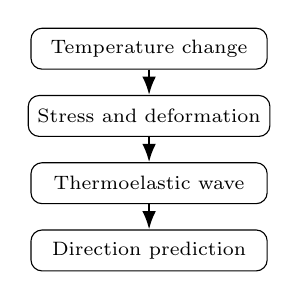
\begin{tikzpicture}[
        node distance=0.32cm,
        box/.style={
          draw,
          rounded corners,
          align=center,
          minimum width=3.0cm,
          minimum height=0.52cm,
          font=\scriptsize
        },
        >=Latex
      ]

        \node[box] (temp) {Temperature change};
        \node[box, below=of temp] (stress) {Stress and deformation};
        \node[box, below=of stress] (wave) {Thermoelastic wave};
        \node[box, below=of wave] (direction) {Direction prediction};

        \draw[->, thick] (temp) -- (stress);
        \draw[->, thick] (stress) -- (wave);
        \draw[->, thick] (wave) -- (direction);

      \end{tikzpicture}

    \end{column}

  \end{columns}
\end{frame}

\begin{frame}{Threats to Validity}
  \begin{enumerate}
    \item \textbf{Limited training data.}
          The COMSOL-derived pilot configuration is not a full calibrated
          geological database.
    \item \textbf{Simplified 2D assumptions.}
          The study uses effective material parameters in a plane-strain setup.
    \item \textbf{FNO normalization issue.}
          The current 2D adaptation is not yet physically reliable.
    \item \textbf{Analytical reference is isotropic.}
          $r/V_p$ is a useful sanity check, not a complete thermoelastic validation.
  \end{enumerate}
\end{frame}

\begin{frame}{Geological Media We Model}
  \begin{columns}[T]
    \begin{column}{0.58\textwidth}
      \footnotesize
      \renewcommand{\arraystretch}{1.20}
      \setlength{\tabcolsep}{4pt}
      \begin{tabular}{l|r|r|r|r|r}
        \hline
        \textbf{Rock} & $\rho$ & $V_P$ & $k$ & $C_p$ & $\alpha$ \\
        & kg/m$^3$ & m/s & W/(m K) & J/(kg K) & $10^{-6}$/K \\
        \hline
        Granite    & 2650 & 5850 & 2.50 &  850 &  7.9 \\
        Basalt     & 3000 & 6550 & 1.95 & 1300 &  --  \\
        Sandstone  & 2725 & 5000 & 2.25 & 1000 & 11.6 \\
        Limestone  & 2675 & 5400 & 2.55 & 1050 &  8.0 \\
        \hline
      \end{tabular}
      \vskip 6pt
      \scriptsize
      Effective scalar parameters under a locally homogeneous isotropic
      approximation; field calibration is out of scope. Full 10-rock tables
      with $E$, $\nu$, $\mu$, $K$, porosity are in the backup slides.
    \end{column}
    \begin{column}{0.40\textwidth}
      \centering
      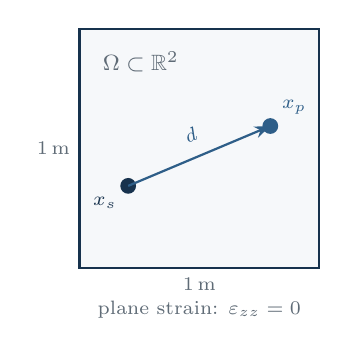
\begin{tikzpicture}[scale=0.95]
        % 2D plane-strain domain illustration
        \draw[thick, fill=AcademicPanel, draw=AcademicNavy]
          (0,0) rectangle (3.2,3.2);
        % Domain label in the top-left corner, clear of the arrow
        \node[AcademicMuted, font=\footnotesize, anchor=north west]
          at (0.18,3.02) {$\Omega \subset \mathbb{R}^{2}$};
        \node[AcademicMuted, font=\scriptsize, below] at (1.6,0)
          {$1$\,m};
        \node[AcademicMuted, font=\scriptsize, left] at (0,1.6)
          {$1$\,m};
        % Source point (label below left, clear of the arrow start)
        \fill[AcademicNavy] (0.65,1.10) circle (3pt);
        \node[AcademicNavy, font=\scriptsize, below left=1pt]
          at (0.65,1.10) {$x_{s}$};
        % Probe point (label above right, clear of the arrow end)
        \fill[AcademicBlue] (2.55,1.90) circle (3pt);
        \node[AcademicBlue, font=\scriptsize, above right=1pt]
          at (2.55,1.90) {$x_{p}$};
        % Direction arrow, label above the line midway
        \draw[->, >={Stealth[length=2mm]}, thick, AcademicBlue]
          (0.65,1.10) -- (2.55,1.90)
          node[midway, above=2pt, sloped, font=\scriptsize] {$d$};
        % Plane strain note
        \node[AcademicMuted, font=\scriptsize] at (1.6,-0.55)
          {plane strain: $\varepsilon_{zz} = 0$};
      \end{tikzpicture}
      \vskip 4pt
      \scriptsize 2D plane-strain domain with source--probe geometry.
    \end{column}
  \end{columns}
\end{frame}

\begin{frame}{Coupled Thermoelastic System}
  \setlength{\abovedisplayskip}{2pt}
  \setlength{\belowdisplayskip}{2pt}
  \setlength{\abovedisplayshortskip}{2pt}
  \setlength{\belowdisplayshortskip}{2pt}
  \begin{columns}[T]
    \begin{column}{0.66\textwidth}
      \begin{block}{Constitutive law (Duhamel--Neumann)}
        \[
          \sigma_{ij} = \lambda\,\delta_{ij}\,\varepsilon_{kk}
                     + 2\mu\,\varepsilon_{ij}
                     - \gamma\,\delta_{ij}\,\theta,
          \quad
          \gamma = 3K\alpha,
          \quad
          \theta = T - T_{0}
        \]
      \end{block}
      \vspace{-4pt}
      \begin{block}{Equation of motion}
        \[
          \rho\,\frac{\partial^{2}u_{i}}{\partial t^{2}}
            = \frac{\partial \sigma_{ij}}{\partial x_{j}} + f_{i}
        \]
      \end{block}
      \vspace{-4pt}
      \begin{block}{Coupled heat equation}
        \[
          \rho C_{p}\,\frac{\partial T}{\partial t}
            - k\,\nabla^{2}T
            + \gamma T_{0}\,\frac{\partial}{\partial t}(\nabla\!\cdot u) = Q
        \]
      \end{block}
      \scriptsize
      $\sigma$ stress; $\varepsilon$ strain; $\lambda,\mu,K$ moduli;
      $\gamma=3K\alpha$ coupling; $\theta=T-T_{0}$; $Q$ heat source.
    \end{column}
    \begin{column}{0.32\textwidth}
      \centering
      \includegraphics[width=\linewidth,height=0.185\textheight,keepaspectratio]{img/wiki_thermal_expansion}\\
      {\scriptsize Thermal expansion $\varepsilon_{\mathrm{th}}=\alpha\Delta T$}\\[2pt]
      \includegraphics[width=0.72\linewidth,height=0.185\textheight,keepaspectratio]{img/wiki_body_waves}\\
      {\scriptsize Elastic body waves (motion)}\\[2pt]
      \includegraphics[width=\linewidth,height=0.135\textheight,keepaspectratio]{img/wiki_heat_conduction}\\
      {\scriptsize Heat flux $q=-k\nabla T$}
    \end{column}
  \end{columns}
\end{frame}

\begin{frame}{2D Directional Prediction Task}
  \begin{columns}[T]
    \begin{column}{0.52\textwidth}
      \centering
      \includegraphics[width=\textwidth]{img/web_visualization}
    \end{column}
    \begin{column}{0.46\textwidth}
      \begin{block}{Scope}
        \footnotesize
        Domain $\Omega \subset \mathbb{R}^{2}$, plane strain, linear
        isotropic thermoelasticity, small deformation. Primary fields are
        the temperature $T(x,t)$ and the in-plane displacement
        $u(x,t) = (u,v)$.
      \end{block}
      \begin{block}{Directional query}
        \[
          d = x_{p} - x_{s},
          \quad
          L = \|d\|,
          \quad
          \hat d = \frac{d}{L}
        \]
        \[
          \phi = \operatorname{atan2}(d_{y}, d_{x}),
          \qquad
          \mathcal{F}: X \to \widehat{Y}
        \]
      \end{block}
      \scriptsize
      $x_{s},x_{p}$ source and probe positions [m];
      $L$ distance [m]; $\hat d$ unit direction; $\phi$ azimuth [rad].
      $\mathcal{F}$ maps input features $X$ (material, geometry, time)
      to the predicted response $\widehat{Y}$ (temperature, displacement,
      directional summary).
    \end{column}
  \end{columns}
\end{frame}

\section{Prediction Framework}

\begin{frame}{COMSOL-Based Synthetic Dataset}
  \begin{columns}[T]
    \begin{column}{0.62\textwidth}
      \centering
      \includegraphics[
        width=\textwidth,
        height=0.68\textheight,
        keepaspectratio
      ]{img/comsol_interface_2d.png}
    \end{column}

    \begin{column}{0.35\textwidth}
      \footnotesize
      \begin{block}{COMSOL simulation}
        The synthetic dataset was generated in COMSOL Multiphysics using a
        coupled thermoelastic model.
      \end{block}

      \begin{itemize}
        \item 2D plane-strain geological domain
        \item Domain size: $1\,\mathrm{m}\times1\,\mathrm{m}$
        \item Initial temperature: $293.15\,\mathrm{K}$
        \item Source temperature: $1500\,\mathrm{K}$
        \item Exported fields: $T$, $(u,v)$, stress, strain, velocity
      \end{itemize}
    \end{column}
  \end{columns}

  \vskip 2pt
  \scriptsize
  The exported COMSOL fields are used as synthetic reference data for comparing
  neural surrogate models.
\end{frame}


\begin{frame}{COMSOL 2D Model and Mesh}
  \begin{columns}[T]
    \begin{column}{0.58\textwidth}
      \centering
      \includegraphics[
        width=\textwidth,
        height=0.70\textheight,
        keepaspectratio
      ]{img/mesh_2d.png}
    \end{column}

    \begin{column}{0.38\textwidth}
      \footnotesize
      \begin{block}{Model domain}
        The numerical experiment represents a two-dimensional section of a
        geological medium with an internal heated source.
      \end{block}

      \begin{block}{Mesh refinement}
        The mesh is refined near the source, where the strongest temperature,
        displacement, and stress gradients are expected.
      \end{block}

      \begin{block}{Role in the study}
        This mesh defines the spatial structure from which the COMSOL fields
        are exported for further preprocessing.
      \end{block}
    \end{column}
  \end{columns}
\end{frame}

\begin{frame}{COMSOL Simulation Results}
  \begin{columns}[T,onlytextwidth]

    \begin{column}{0.332\textwidth}
      \centering
      \includegraphics[
        width=\textwidth,
        height=0.60\textheight,
        trim=0 0 0 32,
        clip,
        keepaspectratio
      ]{img/comsol_temperature_2d.png}

      \vspace{1mm}
      {\scriptsize Local heating creates a compact temperature disturbance
      near the source.}
    \end{column}

    \begin{column}{0.332\textwidth}
      \centering
      \includegraphics[
        width=\textwidth,
        height=0.60\textheight,
        trim=0 0 0 32,
        clip,
        keepaspectratio
      ]{img/comsol_displacement_2d.png}

      \vspace{1mm}
      {\scriptsize Thermal expansion produces a displacement field
      around the heated region.}
    \end{column}

    \begin{column}{0.332\textwidth}
      \centering
      \includegraphics[
        width=\textwidth,
        height=0.60\textheight,
        trim=0 0 0 32,
        clip,
        keepaspectratio
      ]{img/comsol_stress_2d.png}

      \vspace{1mm}
      {\scriptsize The stress field is concentrated near the localized
      thermal source.}
    \end{column}

  \end{columns}
\end{frame}

\begin{frame}{Data Representation and Preprocessing}
  \begin{itemize}
    \item COMSOL simulation results are exported as CSV files for each field
          and time step.
    \item The exported data are aligned into a common node-based representation.
    \item Dynamic fields are assembled into a spatio-temporal tensor:
          \[
            \mathbf{S}\in\mathbb{R}^{N_t \times N_p \times F_d}
          \]
    \item Static material and geometric features are stored separately.
    \item All feature channels are normalized before model training:
          \[
            \widetilde{x}=\frac{x-\mu}{\sigma+\varepsilon}
          \]
  \end{itemize}

  \scriptsize
  Here, $N_t$ is the number of time steps, $N_p$ is the number of spatial
  points, and $F_d$ is the number of dynamic physical fields. The same processed
  dataset is then reused by coordinate-based, grid-based, and graph-based
  neural models.
\end{frame}

\section{Comparative Framework}

\begin{frame}{Comparative Prototype Framework}
  \begin{block}{One workflow for all model routes}
    The frontend, backend orchestrator, material catalog, and model
    services use one shared input--output contract for fair comparison.
  \end{block}
  \vskip 6pt
  \begin{itemize}
    \item Same source--probe geometry for all routes
    \item Same effective geological material presets
    \item Same normalized response format: temperature, displacement,
          direction, travel time, and diagnostics
  \end{itemize}
\end{frame}

\begin{frame}{Shared Model Comparison Contract}
  \begin{block}{Common interpretation}
    All routes are treated as surrogate modelling approaches for the same
    AI-Guided Prediction of Thermoelastic Wave Propagation in Geological Media
    task, not as complete numerical solvers.
  \end{block}
  \begin{columns}[T]
    \begin{column}{0.32\textwidth}
      \begin{block}{Input}
        \footnotesize
        Material parameters, source--probe geometry, observation time, and
        processed field features.
      \end{block}
    \end{column}
    \begin{column}{0.32\textwidth}
      \begin{block}{Output}
        \footnotesize
        Estimated temperature, displacement components, travel time, and
        diagnostic response quantities.
      \end{block}
    \end{column}
    \begin{column}{0.32\textwidth}
      \begin{block}{Comparison basis}
        \footnotesize
        Same material presets, geometry contract, response format, and
        analytical travel-time sanity check.
      \end{block}
    \end{column}
  \end{columns}
\end{frame}

\begin{frame}{Implementation Stack}
  \begin{columns}[T,onlytextwidth]
    \begin{column}{0.47\textwidth}
      \begin{block}{Local thesis-demo stack}
        \footnotesize
        The prototype is packaged as a local Docker Compose workspace with
        a FastAPI orchestration backend, a native web frontend, and separate
        Python model services.
      \end{block}
      \vspace{2mm}
      \footnotesize
      \begin{itemize}
        \item \textbf{Frontend:} HTML, CSS, JavaScript interface for scenario setup.
        \item \textbf{Backend:} FastAPI validates requests and normalizes responses.
        \item \textbf{Services:} Python inference endpoints for PINN, FNO,
              MeshGraphNet, and Transformer routes.
        \item \textbf{Deployment:} Docker Compose starts the demo stack locally.
      \end{itemize}
    \end{column}
    \begin{column}{0.49\textwidth}
      \centering
      \resizebox{!}{0.49\textheight}{%
      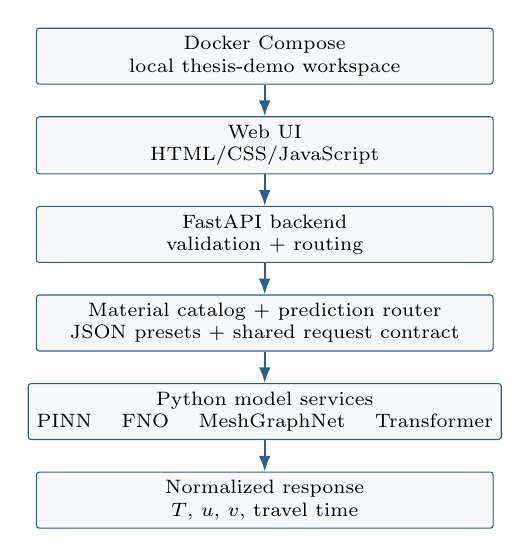
\begin{tikzpicture}[
        font=\scriptsize,
        node distance=4mm and 7mm,
        box/.style={
          draw=AcademicBlue,
          fill=AcademicPanel,
          rounded corners=1pt,
          align=center,
          inner sep=3pt,
          minimum width=58mm,
          minimum height=7mm
        },
        service/.style={
          draw=AcademicNavy,
          fill=white,
          rounded corners=1pt,
          align=center,
          inner sep=3pt,
          minimum width=30mm,
          minimum height=7mm
        },
        arrow/.style={-{Latex[length=2mm]}, thick, draw=AcademicBlue}
      ]
        \node[box] (docker) {Docker Compose\\local thesis-demo workspace};
        \node[box, below=of docker] (ui) {Web UI\\HTML/CSS/JavaScript};
        \node[box, below=of ui] (api) {FastAPI backend\\validation + routing};
        \node[box, below=of api] (catalog) {Material catalog + prediction router\\JSON presets + shared request contract};
        \node[box, below=of catalog] (models) {Python model services\\
          PINN \quad FNO \quad MeshGraphNet \quad Transformer};
        \node[box, below=of models] (out) {Normalized response\\$T$, $u$, $v$, travel time};

        \draw[arrow] (docker) -- (ui);
        \draw[arrow] (ui) -- (api);
        \draw[arrow] (api) -- (catalog);
        \draw[arrow] (catalog) -- (models);
        \draw[arrow] (models) -- (out);
      \end{tikzpicture}}
      \vspace{2mm}

      {\scriptsize The backend does not replace the models; it orchestrates
      model-specific services and returns one comparable response format.}
    \end{column}
  \end{columns}
\end{frame}

\begin{frame}{PINN: Physics-Informed Baseline}
  \begin{columns}[T]
    \begin{column}{0.50\textwidth}
      \begin{block}{Role in the framework}
        \footnotesize
        PINN is the explicitly physics-informed route in the comparison.
      \end{block}
      \begin{itemize}
        \footnotesize
        \item Uses supervised data and thermoelastic residuals.
        \item Predicts temperature and displacement fields.
        \item Serves as the physics-informed baseline for data-driven routes.
      \end{itemize}
    \end{column}
    \begin{column}{0.46\textwidth}
      \begin{alertblock}{Interpretation}
        \footnotesize
        PINN is a neural surrogate whose loss encourages physical consistency.
        It is not an exact numerical solver.
      \end{alertblock}
      \begin{block}{Practical setup}
        \footnotesize
        Used in the simplified 2D source--probe prediction workflow.
      \end{block}
    \end{column}
  \end{columns}
\end{frame}

\begin{frame}[shrink=5]{PINN Input and Architecture}
  \begin{block}{Public neural contract}
    \[
      [x,y,t,E,\nu,\rho,\alpha,k,C_p]\rightarrow[T,u,v]
    \]
  \end{block}
  \begin{columns}[T]
    \begin{column}{0.56\textwidth}
      \centering
      \resizebox{!}{0.34\textheight}{%
      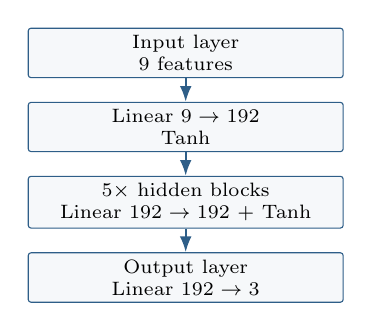
\begin{tikzpicture}[
        font=\scriptsize,
        node distance=3mm,
        box/.style={draw=AcademicBlue, fill=AcademicPanel, rounded corners=1pt,
          align=center, inner sep=2.5pt, minimum height=6mm, minimum width=40mm},
        arrow/.style={-{Latex[length=2mm]}, thick, draw=AcademicBlue}
      ]
        \node[box] (inp) {Input layer\\$9$ features};
        \node[box, below=of inp] (h1) {Linear $9 \rightarrow 192$\\Tanh};
        \node[box, below=of h1] (hrep) {$5 \times$ hidden blocks\\Linear $192 \rightarrow 192$ + Tanh};
        \node[box, below=of hrep] (out) {Output layer\\Linear $192 \rightarrow 3$};
        \draw[arrow] (inp) -- (h1);
        \draw[arrow] (h1) -- (hrep);
        \draw[arrow] (hrep) -- (out);
      \end{tikzpicture}
      }
    \end{column}
    \begin{column}{0.40\textwidth}
      {\scriptsize\textbf{Implemented network.} \texttt{MLP\_PINN},
      hidden dimension $192$, depth $6$, default activation \texttt{tanh}.}
      \begin{block}{Input features}
        \scriptsize
        \begin{tabular}{@{}ll@{}}
          $x,y,t$ & geometry and time\\
          $E,\nu$ & elastic parameters\\
          $\rho$ & density\\
          $\alpha,k,C_p$ & thermal parameters
        \end{tabular}
      \end{block}
      {\scriptsize\textbf{Output features.}
      $\hat{Y}=[\hat{T},\hat{u},\hat{v}]$.
      Temperature and two in-plane displacement components are predicted.
      Velocity, stress, and strain are derived through autograd during residual
      and velocity-consistency evaluation.}
    \end{column}
  \end{columns}
\end{frame}

\begin{frame}{PINN Composite Loss and Residuals}
  \begin{block}{Hybrid training objective}
    \[
      \mathcal{L}
      =
      \lambda_{\mathrm{sup}}\mathcal{L}_{\mathrm{sup}}
      +
      \lambda_{\mathrm{vel}}\mathcal{L}_{\mathrm{vel}}
      +
      \lambda_{\mathrm{wave}}\mathcal{L}_{\mathrm{wave}}
      +
      \lambda_{\mathrm{th}}\mathcal{L}_{\mathrm{th}}
    \]
  \end{block}
  \begin{columns}[T]
    \begin{column}{0.50\textwidth}
      \footnotesize
      \begin{itemize}
        \item $\mathcal{L}_{\mathrm{sup}}$: supervised field loss for
              $T,u,v$.
        \item $\mathcal{L}_{\mathrm{vel}}$: velocity consistency from time
              derivatives.
        \item $\mathcal{L}_{\mathrm{wave}}$: elastic wave residual.
        \item $\mathcal{L}_{\mathrm{th}}$: coupled thermal residual.
      \end{itemize}
    \end{column}
    \begin{column}{0.46\textwidth}
      \begin{alertblock}{Current limitation}
        \footnotesize
        Dedicated boundary-condition and initial-condition losses are not yet
        enforced.
      \end{alertblock}
      \scriptsize
      In the implemented 2D mode, strain, stress, wave residual, and coupled
      thermal residual are computed from automatic derivatives.
    \end{column}
  \end{columns}
\end{frame}

\begin{frame}{Fourier Neural Operator}
  \begin{columns}
    \begin{column}{0.50\textwidth}
      \begin{block}{Operator view}
        \[
          \mathcal{G}_{\theta}:\mathcal{A}\rightarrow\mathcal{U},
          \qquad
          \hat{s}=\mathcal{G}_{\theta}(a)
        \]
      \end{block}
      \begin{block}{Input tensor}
        \[
          A\in\mathbb{R}^{B\times C_{in}\times N_x\times N_y}
        \]
      \end{block}
      \begin{block}{Output tensor}
        \[
          \hat{S}\in\mathbb{R}^{B\times C_{out}\times N_x\times N_y}
        \]
      \end{block}
    \end{column}
    \begin{column}{0.46\textwidth}
      \scriptsize
      $a$ -- input field; $\hat{s}$ -- predicted thermoelastic field;
      $\mathcal{A}$ and $\mathcal{U}$ -- input and output field spaces;
      $\theta$ -- trainable neural-operator parameters.
      \footnotesize
      \begin{itemize}
        \item $B$ is batch size.
        \item $N_x,N_y$ are grid sizes.
        \item $C_{in}$ is the number of input channels.
        \item $C_{out}$ is controlled by \texttt{out\_channels}.
      \end{itemize}
      \vskip 4pt
      For the three-channel thermoelastic setup:
      \[
        C_{out}=3,\qquad \hat{s}=[\hat{T},\hat{u},\hat{v}].
      \]
    \end{column}
  \end{columns}
\end{frame}

\begin{frame}{FNO Pipeline}
\centering
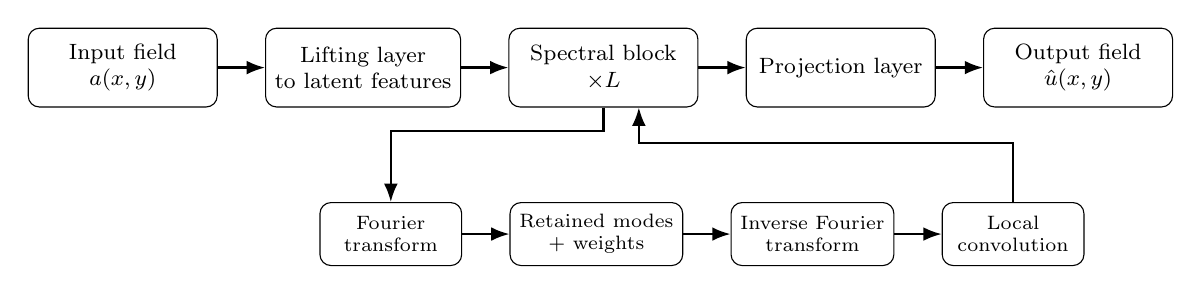
\begin{tikzpicture}[
    node distance=0.9cm and 0.6cm,
    box/.style={
        draw,
        rounded corners,
        align=center,
        minimum width=2.4cm,
        minimum height=1cm,
        font=\footnotesize
    },
    smallbox/.style={
        draw,
        rounded corners,
        align=center,
        minimum width=1.8cm,
        minimum height=0.8cm,
        font=\scriptsize
    },
    >=Latex
]

\node[box] (input) {Input field\\$a(x,y)$};
\node[box, right=of input] (lift) {Lifting layer\\to latent features};
\node[box, right=of lift] (spec) {Spectral block\\$\times L$};
\node[box, right=of spec] (proj) {Projection layer};
\node[box, right=of proj] (out) {Output field\\$\hat{u}(x,y)$};

\draw[->, thick] (input) -- (lift);
\draw[->, thick] (lift) -- (spec);
\draw[->, thick] (spec) -- (proj);
\draw[->, thick] (proj) -- (out);

% inner spectral block
\node[smallbox, below=1.2cm of spec, xshift=-2.7cm] (fft) {Fourier\\transform};
\node[smallbox, right=of fft] (modes) {Retained modes\\+ weights};
\node[smallbox, right=of modes] (ifft) {Inverse Fourier\\transform};
\node[smallbox, right=of ifft] (conv) {Local\\convolution};

\draw[->, thick] (fft) -- (modes);
\draw[->, thick] (modes) -- (ifft);
\draw[->, thick] (ifft) -- (conv);

\draw[->, thick] (spec.south) -- ++(0,-0.3) -| (fft.north);
\draw[->, thick] (conv.north) -- ++(0,0.75) -| ([xshift=0.45cm]spec.south);

\end{tikzpicture}

\vspace{0.4cm}

\footnotesize
FNO maps an input field to an output field by combining
global spectral interactions and local spatial corrections.
\end{frame}

\begin{frame}{FNO Spectral Block}
\begin{columns}[T]
    \begin{column}{0.52\textwidth}
        \begin{block}{Layer update}
        \[
        v_{l+1}=\sigma\left(\mathcal{S}_l(v_l)+\mathcal{C}_l(v_l)\right)
        \]
        \scriptsize
        where \(v_l\) is the latent feature field at layer \(l\);\\
        \(\mathcal{S}_l\) is the spectral branch;\\
        \(\mathcal{C}_l\) is the local convolution branch;\\
        \(\sigma\) is the activation function.
        \end{block}

        \begin{block}{Spectral transform}
        \[
        \hat{v}_l=\mathcal{F}(v_l), \qquad
        z_l=\mathcal{F}^{-1}(R_l\hat{v}_l)
        \]
        \scriptsize
        where \(\mathcal{F}\) is the Fourier transform;\\
        \(\mathcal{F}^{-1}\) is the inverse Fourier transform;\\
        \(R_l\) is the trainable spectral weight tensor.
        \end{block}
    \end{column}

    \begin{column}{0.44\textwidth}
        \footnotesize
        \textbf{Interpretation:}
        \begin{itemize}
            \item Fourier transform moves the field into frequency space.
            \item Only low-frequency modes are retained and transformed.
            \item Inverse transform returns the result to physical space.
            \item Local convolution restores short-range spatial details.
        \end{itemize}

        \vspace{0.3cm}

        \begin{block}{Retained modes}
        \[
        \texttt{modes}=[K_1,K_2], \qquad d=2
        \]
        \scriptsize
        \(K_1,K_2\) are the retained Fourier modes in two spatial directions.
        \end{block}
    \end{column}
\end{columns}
\end{frame}

\begin{frame}{Training and Evaluation of FNO}
\centering

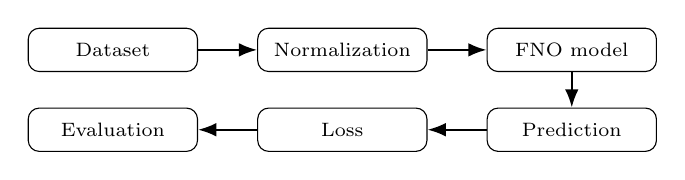
\begin{tikzpicture}[
    node distance=0.45cm and 0.75cm,
    box/.style={
        draw,
        rounded corners,
        align=center,
        minimum width=2.15cm,
        minimum height=0.55cm,
        font=\scriptsize
    },
    >=Latex
]

\node[box] (data) {Dataset};
\node[box, right=of data] (norm) {Normalization};
\node[box, right=of norm] (model) {FNO model};

\node[box, below=of model] (pred) {Prediction};
\node[box, left=of pred] (loss) {Loss};
\node[box, left=of loss] (eval) {Evaluation};

\draw[->, thick] (data) -- (norm);
\draw[->, thick] (norm) -- (model);
\draw[->, thick] (model) -- (pred);
\draw[->, thick] (pred) -- (loss);
\draw[->, thick] (loss) -- (eval);

\end{tikzpicture}

\vspace{0.15cm}

\begin{columns}[T]
    \begin{column}{0.52\textwidth}

        \begin{block}{Training objective}
        \[
        \mathcal{L}=\lambda_{MSE}\mathcal{L}_{MSE}
        +\lambda_{rel}\mathcal{L}_{rel}
        \]
        \scriptsize
        \(\mathcal{L}\) is the total loss;
        \(\mathcal{L}_{MSE}\) measures point-wise field error;
        \(\mathcal{L}_{rel}\) measures relative \(L^2\) deviation;
        \(\lambda_{MSE}\), \(\lambda_{rel}\) control their contribution.
        \end{block}

        \scriptsize
        Normalization is computed on the training set and reused during
        validation, testing, and inference:
        \[
          \tilde{s}_{i,c}=\frac{s_{i,c}-\mu_c}{\sigma_c}.
        \]

    \end{column}

    \begin{column}{0.42\textwidth}

        \footnotesize
        \textbf{Evaluation includes:}
        \scriptsize
        \begin{itemize}
            \item field-level visual comparison;
            \item channel-wise prediction errors;
            \item relative \(L^2\) error;
            \item physical sanity checks.
        \end{itemize}

        \vspace{-2pt}

        \begin{alertblock}{Current caveat}
        \scriptsize
        The FNO prototype is useful as a field-based neural-operator baseline,
        but still requires output-scale recalibration before being treated as
        a physically reliable predictor.
        \end{alertblock}

    \end{column}
\end{columns}

\end{frame}


% Required packages:
% \usepackage{tikz}
% \usetikzlibrary{positioning,fit,arrows.meta,calc}
\begin{frame}[t]{MeshGraphNet: Graph Input and Prediction}
\scriptsize
\vspace{-2mm}
\setlength{\abovedisplayskip}{1pt}
\setlength{\belowdisplayskip}{1pt}

\begin{block}{Main idea}
MeshGraphNet represents the COMSOL mesh as a graph and predicts the next
thermoelastic state at each mesh node.
\end{block}

\vspace{-2mm}

\begin{columns}[T,onlytextwidth]

\begin{column}{0.45\textwidth}
\centering
\resizebox{0.95\linewidth}{!}{%
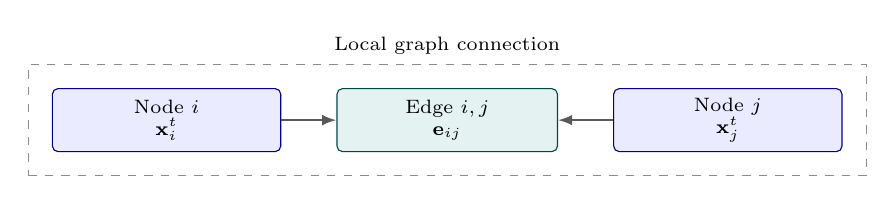
\begin{tikzpicture}[
  font=\scriptsize,
  nodebox/.style={rectangle, rounded corners=2pt,
    draw=blue!55!black, fill=blue!8,
    minimum width=29mm, minimum height=8mm, align=center},
  edgebox/.style={rectangle, rounded corners=2pt,
    draw=teal!55!black, fill=teal!10,
    minimum width=28mm, minimum height=8mm, align=center},
  arr/.style={-{Latex[length=1.8mm]}, thick, draw=black!65}
]

\node[nodebox] (xi) {Node \(i\)\\$\mathbf{x}_i^t$};
\node[edgebox, right=7mm of xi] (eij) {Edge \(i,j\)\\$\mathbf{e}_{ij}$};
\node[nodebox, right=7mm of eij] (xj) {Node \(j\)\\$\mathbf{x}_j^t$};

\draw[arr] (xi) -- (eij);
\draw[arr] (xj) -- (eij);

\node[
  draw=black!45,
  dashed,
  fit=(xi)(eij)(xj),
  inner sep=3mm,
  label={[font=\scriptsize]above:Local graph connection}
] {};

\end{tikzpicture}}

\vspace{1mm}

\begin{block}{Graph}
\[
  \mathcal{G}=(\mathcal{V},\mathcal{E})
\]
\(\mathcal{G}\) -- graph representation;  
\(\mathcal{V}\) -- mesh nodes;  
\(\mathcal{E}\) -- edges between neighbouring nodes.
\end{block}

\end{column}

\begin{column}{0.53\textwidth}

\begin{block}{Node features}
\[
  \mathbf{x}_i^t=
  (\mathbf{p}_i,\mathbf{s}_i^t,\mathbf{m}_i,\mathbf{c})
\]
\(\mathbf{x}_i^t\) -- feature vector of node \(i\) at time \(t\);  
\(\mathbf{p}_i\) -- node position;  
\(\mathbf{s}_i^t\) -- current physical state;  
\(\mathbf{m}_i\) -- material parameters;  
\(\mathbf{c}\) -- scenario condition.
\end{block}

\vspace{-2mm}

\begin{block}{Edge features}
\[
  \mathbf{e}_{ij}=
  [\mathbf{p}_j-\mathbf{p}_i,\|\mathbf{p}_j-\mathbf{p}_i\|]
\]
\(\mathbf{e}_{ij}\) -- edge attribute between nodes \(i\) and \(j\);  
\(\mathbf{p}_j-\mathbf{p}_i\) -- relative position;  
\(\|\mathbf{p}_j-\mathbf{p}_i\|\) -- distance between nodes.
\end{block}

\vspace{-2mm}

\begin{block}{Prediction}
\[
  \hat{\mathbf{y}}_i^{\,t+1}
  =
  F_{\theta}(\mathcal{G},\mathbf{x}^t)_i
\]
\(F_{\theta}\) -- trained MeshGraphNet model;  
\(\hat{\mathbf{y}}_i^{\,t+1}\) -- predicted physical fields for node \(i\).
\end{block}

\end{column}
\end{columns}
\end{frame}
\begin{frame}{MeshGraphNet: Encoder--Processor--Decoder}
  \centering
  \resizebox{!}{0.74\textheight}{%
  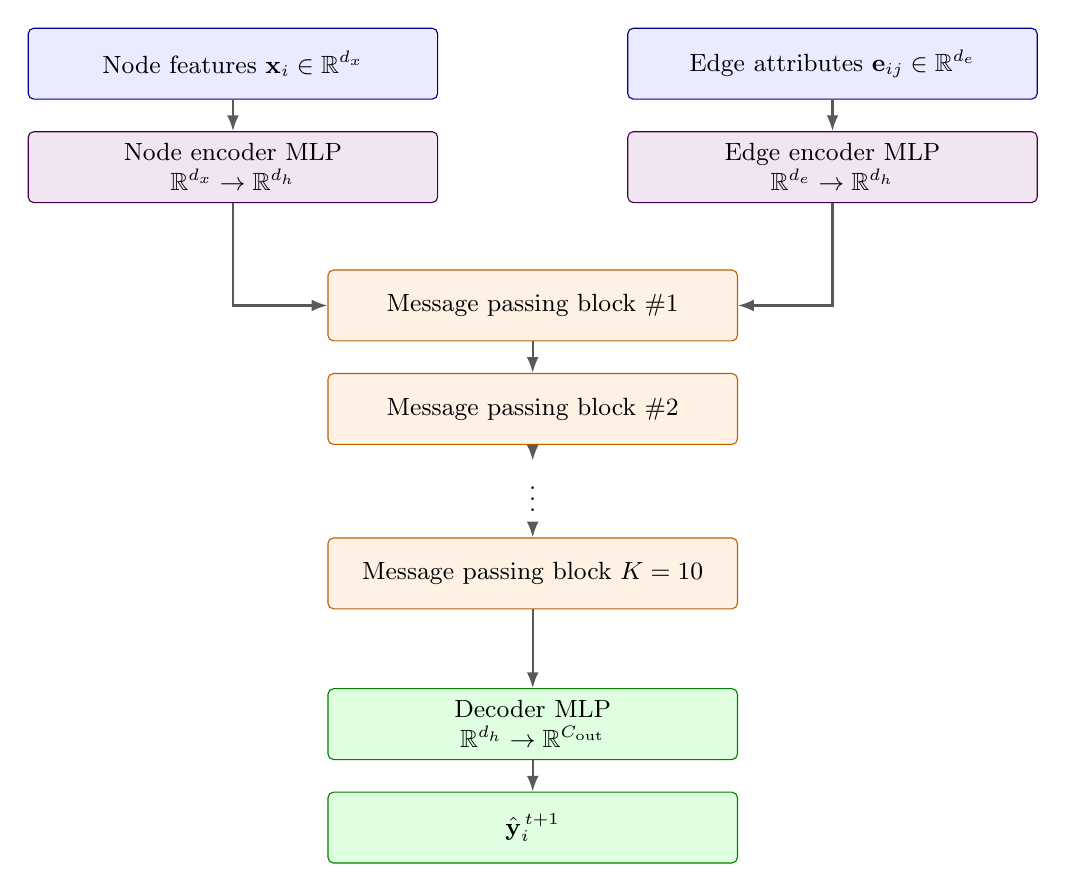
\begin{tikzpicture}[
    font=\small,
    node distance=4mm and 14mm,
    inp/.style={rectangle, rounded corners=2pt,
      draw=blue!55!black, fill=blue!8,
      minimum width=52mm, minimum height=9mm, align=center},
    enc/.style={rectangle, rounded corners=2pt,
      draw=violet!55!black, fill=violet!10,
      minimum width=52mm, minimum height=9mm, align=center},
    proc/.style={rectangle, rounded corners=2pt,
      draw=orange!75!black, fill=orange!10,
      minimum width=52mm, minimum height=9mm, align=center},
    outp/.style={rectangle, rounded corners=2pt,
      draw=green!50!black, fill=green!12,
      minimum width=52mm, minimum height=9mm, align=center},
    arr/.style={-{Latex[length=2mm]}, thick, draw=black!65}
  ]
    \node[inp] (xin) {Node features \(\mathbf{x}_i\in\mathbb{R}^{d_x}\)};
    \node[inp, right=24mm of xin] (ein) {Edge attributes \(\mathbf{e}_{ij}\in\mathbb{R}^{d_e}\)};

    \node[enc, below=of xin] (nenc) {Node encoder MLP\\ \(\mathbb{R}^{d_x}\to\mathbb{R}^{d_h}\)};
    \node[enc, below=of ein] (eenc) {Edge encoder MLP\\ \(\mathbb{R}^{d_e}\to\mathbb{R}^{d_h}\)};

    \node[proc, below=13mm of $(nenc)!0.5!(eenc)$] (p1) {Message passing block \#1};
    \node[proc, below=of p1] (p2) {Message passing block \#2};
    \node[below=2mm of p2] (pdots) {\(\vdots\)};
    \node[proc, below=2mm of pdots] (pK) {Message passing block \(K=10\)};

    \node[outp, below=10mm of pK] (dec) {Decoder MLP\\ \(\mathbb{R}^{d_h}\to\mathbb{R}^{C_{\mathrm{out}}}\)};
    \node[outp, below=of dec] (yhat) {\(\hat{\mathbf{y}}_i^{\,t+1}\)};

    \draw[arr] (xin) -- (nenc);
    \draw[arr] (ein) -- (eenc);
    \draw[arr] (nenc.south) |- (p1.west);
    \draw[arr] (eenc.south) |- (p1.east);
    \draw[arr] (p1) -- (p2);
    \draw[arr] (p2) -- (pdots);
    \draw[arr] (pdots) -- (pK);
    \draw[arr] (pK) -- (dec);
    \draw[arr] (dec) -- (yhat);
  \end{tikzpicture}}

  \vskip 2pt
  {\scriptsize The model uses latent dimension \(d_h=128\), ten message-passing steps, MLP encoders, and a node-wise decoder.}
\end{frame}

\begin{frame}{MeshGraphNet: Encoder and Decoder}
\scriptsize

\begin{columns}[T,onlytextwidth]

\begin{column}{0.48\textwidth}
\begin{block}{Encoder}
\[
  \mathbf{h}_i^0 = \phi_v^{enc}(\mathbf{x}_i^t),
  \qquad
  \mathbf{g}_{ij}^0 = \phi_e^{enc}(\mathbf{e}_{ij})
\]

The encoder transforms raw node and edge information into latent vectors.

\vspace{1mm}

\(\mathbf{x}_i^t\) is the node feature vector,  
\(\mathbf{e}_{ij}\) is the edge feature vector,  
\(\mathbf{h}_i^0\) is the initial latent node embedding,  
\(\mathbf{g}_{ij}^0\) is the initial latent edge embedding.
\end{block}
\end{column}

\begin{column}{0.48\textwidth}
\begin{block}{Decoder}
\[
  \hat{\mathbf{y}}_i^{\,t+1}
  =
  \phi^{dec}(\mathbf{h}_i^K)
\]

The decoder converts the final latent node embedding into predicted physical
fields for the next time step.

\vspace{1mm}

\(\mathbf{h}_i^K\) is the node embedding after \(K\) message-passing steps,  
\(\hat{\mathbf{y}}_i^{\,t+1}\) is the predicted output vector.
\end{block}
\end{column}

\end{columns}

\vspace{2mm}

\begin{block}{Implementation detail}
Both encoders and the decoder are implemented as MLPs. In the current
MeshGraphNet configuration, the latent dimension is \(d_h=128\), and the
processor applies \(K=10\) message-passing steps.
\end{block}

\end{frame}

\begin{frame}{MeshGraphNet: Message Passing Block}
  \setlength{\abovedisplayskip}{2pt}
  \setlength{\belowdisplayskip}{2pt}

  \begin{block}{Edge update}
    \[
      \mathbf{e}_{ij}' =
      \operatorname{LN}\Big(
      \mathbf{e}_{ij}+
      \phi_e([\mathbf{h}_i,\mathbf{h}_j,\mathbf{e}_{ij}])
      \Big)
    \]
  \end{block}

  \begin{columns}[T]
    \begin{column}{0.48\textwidth}
      \begin{block}{Aggregation}
        \scriptsize
        \[
          \mathbf{a}_j =
          \sum_{i:(i,j)\in\mathcal{E}}
          \mathbf{e}_{ij}'
        \]
        Incoming edge messages are accumulated for every destination node
        using scatter-add aggregation.
      \end{block}
    \end{column}

    \begin{column}{0.48\textwidth}
      \begin{block}{Node update}
        \scriptsize
        \[
          \mathbf{h}_j' =
          \operatorname{LN}\Big(
          \mathbf{h}_j+
          \phi_v([\mathbf{h}_j,\mathbf{a}_j])
          \Big)
        \]
        The residual connection preserves the previous node state and improves
        stability during repeated message passing.
      \end{block}
    \end{column}
  \end{columns}

  \vskip 4pt
  \scriptsize
  Here \(\phi_e\) and \(\phi_v\) are MLPs with Linear layers, LayerNorm,3
  SiLU activation, and optional Dropout.
\end{frame}
\begin{frame}{Transformer: Inputs and Outputs}
  \begin{columns}[T]
    \begin{column}{0.60\textwidth}
      \centering
      \resizebox{\linewidth}{!}{%
      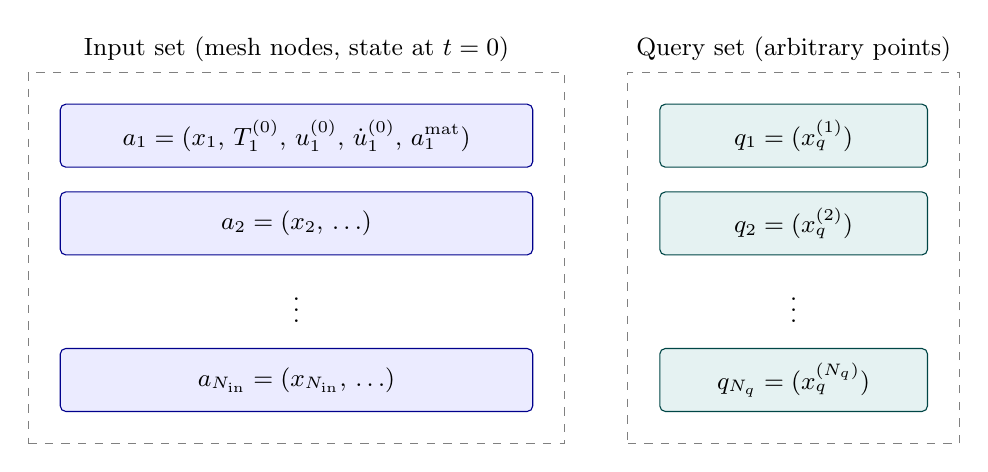
\begin{tikzpicture}[
        font=\small,
        node distance=3mm and 12mm,
        itok/.style={rectangle, rounded corners=2pt,
          draw=blue!55!black, fill=blue!8,
          minimum width=60mm, minimum height=8mm, inner sep=3pt, align=left},
        qtok/.style={rectangle, rounded corners=2pt,
          draw=teal!55!black, fill=teal!10,
          minimum width=34mm, minimum height=8mm, inner sep=3pt, align=left}
      ]
        \node[itok] (i1) {$a_1=(x_1,\,T_1^{(0)},\,u_1^{(0)},\,\dot u_1^{(0)},\,a_1^{\text{mat}})$};
        \node[itok, below=of i1] (i2) {$a_2=(x_2,\,\ldots)$};
        \node[below=2mm of i2] (idots) {$\vdots$};
        \node[itok, below=2mm of idots] (iN) {$a_{N_{\mathrm{in}}}=(x_{N_{\mathrm{in}}},\,\ldots)$};
        \node[draw=black!50, dashed, fit=(i1)(iN), inner sep=4mm,
          label=above:{Input set (mesh nodes, state at $t=0$)}] {};
        \node[qtok, right=16mm of i1.east] (q1) {$q_1=(x_q^{(1)})$};
        \node[qtok, below=of q1] (q2) {$q_2=(x_q^{(2)})$};
        \node[below=2mm of q2] (qdots) {$\vdots$};
        \node[qtok, below=2mm of qdots] (qN) {$q_{N_q}=(x_q^{(N_q)})$};
        \node[draw=black!50, dashed, fit=(q1)(qN), inner sep=4mm,
          label=above:{Query set (arbitrary points)}] {};
      \end{tikzpicture}}
    \end{column}
    \begin{column}{0.38\textwidth}
      \footnotesize
      \begin{block}{Input token \(\in\mathbb{R}^{13}\)}
        coordinates, initial state \((T,u,v,\dot u,\dot v)\), and material
        parameters \((E,\nu,\rho,\alpha,k,C_p)\).
      \end{block}
      \begin{block}{Query token \(\in\mathbb{R}^{2}\)}
        the coordinates \(q_j=(x_q^{(j)},y_q^{(j)})\) where fields are
        requested.
      \end{block}
      \begin{block}{Output \(\in\mathbb{R}^{3}\)}
        \[ \hat y_j = (\hat T_j,\,\hat u_j,\,\hat v_j) \]
      \end{block}
      \scriptsize
      \(N_{\mathrm{in}}\) and \(N_q\) are independent, so the operator is
      discretisation-invariant.
    \end{column}
  \end{columns}
\end{frame}

\begin{frame}{Transformer: Architecture}
  \centering
  \resizebox{!}{0.72\textheight}{%
  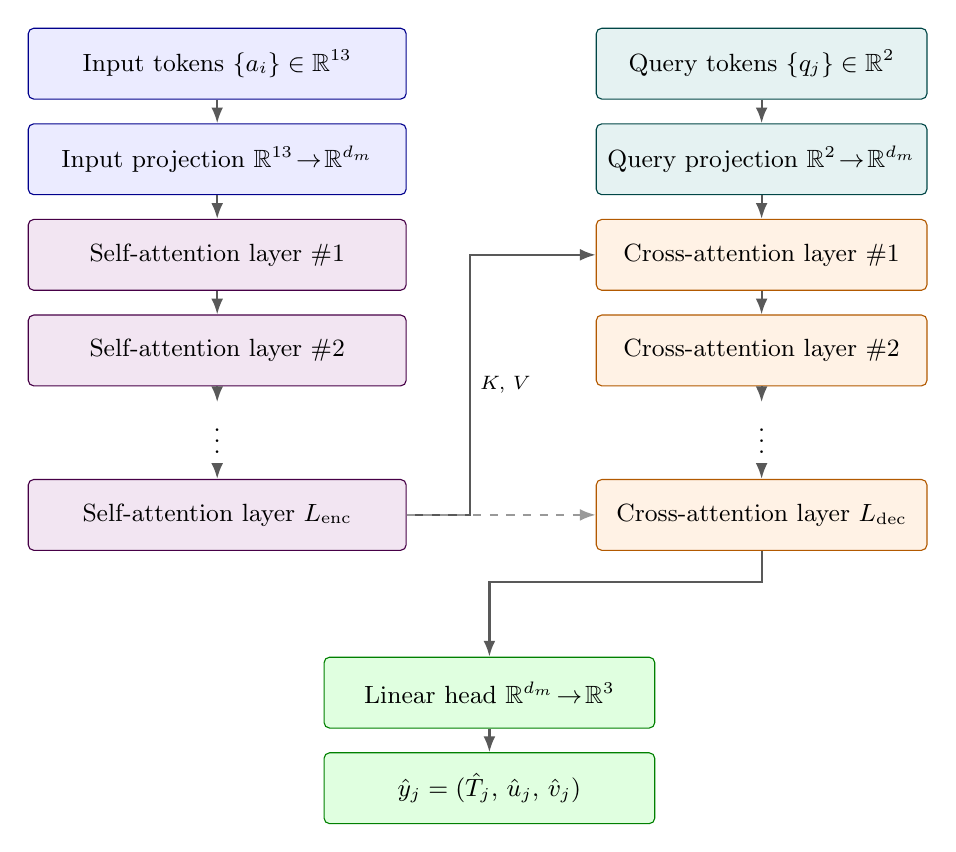
\begin{tikzpicture}[
    font=\small,
    node distance=3mm and 12mm,
    inp/.style={rectangle, rounded corners=2pt,
      draw=blue!55!black, fill=blue!8,
      minimum width=48mm, minimum height=9mm, align=center},
    enc/.style={rectangle, rounded corners=2pt,
      draw=violet!55!black, fill=violet!10,
      minimum width=48mm, minimum height=9mm, align=center},
    qry/.style={rectangle, rounded corners=2pt,
      draw=teal!55!black, fill=teal!10,
      minimum width=42mm, minimum height=9mm, align=center},
    dec/.style={rectangle, rounded corners=2pt,
      draw=orange!70!black, fill=orange!10,
      minimum width=42mm, minimum height=9mm, align=center},
    outp/.style={rectangle, rounded corners=2pt,
      draw=green!50!black, fill=green!12,
      minimum width=42mm, minimum height=9mm, align=center},
    arr/.style={-{Latex[length=2mm]}, thick, draw=black!65}
  ]
    \node[inp] (in)   {Input tokens \(\{a_i\}\in\mathbb{R}^{13}\)};
    \node[inp, below=of in] (ip) {Input projection \(\mathbb{R}^{13}\!\to\!\mathbb{R}^{d_m}\)};
    \node[enc, below=of ip] (e1) {Self-attention layer \#1};
    \node[enc, below=of e1] (e2) {Self-attention layer \#2};
    \node[below=2mm of e2] (edots) {\(\vdots\)};
    \node[enc, below=2mm of edots] (eL) {Self-attention layer \(L_{\mathrm{enc}}\)};

    \node[qry, right=24mm of in] (q)  {Query tokens \(\{q_j\}\in\mathbb{R}^{2}\)};
    \node[qry, below=of q]   (qp) {Query projection \(\mathbb{R}^{2}\!\to\!\mathbb{R}^{d_m}\)};
    \node[dec, below=of qp]  (d1) {Cross-attention layer \#1};
    \node[dec, below=of d1]  (d2) {Cross-attention layer \#2};
    \node[below=2mm of d2]   (ddots) {\(\vdots\)};
    \node[dec, below=2mm of ddots] (dL) {Cross-attention layer \(L_{\mathrm{dec}}\)};

    \node[outp, below=18mm of $(eL)!0.5!(dL)$] (head) {Linear head \(\mathbb{R}^{d_m}\!\to\!\mathbb{R}^{3}\)};
    \node[outp, below=of head] (yhat) {\(\hat{y}_j = (\hat T_j,\,\hat u_j,\,\hat v_j)\)};

    \draw[arr] (in) -- (ip);
    \draw[arr] (ip) -- (e1);
    \draw[arr] (e1) -- (e2);
    \draw[arr] (e2) -- (edots);
    \draw[arr] (edots) -- (eL);

    \draw[arr] (q)  -- (qp);
    \draw[arr] (qp) -- (d1);
    \draw[arr] (d1) -- (d2);
    \draw[arr] (d2) -- (ddots);
    \draw[arr] (ddots) -- (dL);

    \draw[arr] (eL.east) -- ++(8mm,0) |- (d1.west) node[pos=0.25, right] {\scriptsize \(K,\,V\)};
    \draw[arr, dashed, draw=black!40] (eL.east) -- ++(8mm,0) |- (dL.west);

    \draw[arr] (dL.south) -- ++(0,-4mm) -| (head.north);
    \draw[arr] (head) -- (yhat);
  \end{tikzpicture}}

  \vskip 2pt
  {\scriptsize Encoder self-attention; decoder cross-attention from queries;
   linear head returns \((T,u,v)\).}
\end{frame}

\begin{frame}{Transformer: Training Loss}
  \setlength{\abovedisplayskip}{2pt}
  \setlength{\belowdisplayskip}{2pt}
  \setlength{\abovedisplayshortskip}{1pt}
  \setlength{\belowdisplayshortskip}{1pt}
  \begin{block}{Composite objective}
    \[
      \mathcal{L}(\theta)=
      \lambda_{\mathrm{sup}}\mathcal{L}_{\mathrm{sup}}
      +\lambda_{\mathrm{vel}}\mathcal{L}_{\mathrm{vel}}
      +\lambda_{\mathrm{th}}\mathcal{L}_{\mathrm{th}},
      \qquad
      (\lambda_{\mathrm{sup}},\lambda_{\mathrm{vel}},\lambda_{\mathrm{th}})
      =(1.0,\,0.25,\,0.05)
    \]
  \end{block}
  \begin{columns}[T]
    \begin{column}{0.33\textwidth}
      \begin{block}{Supervised (data)}
        \scriptsize
        \[
          \mathcal{L}_{\mathrm{sup}}=
          \frac{1}{N_q C_{\mathrm{out}}}
          \sum_{j,c}\big(\hat y_{j,c}-y_{j,c}\big)^2
        \]
        Reconstructs the COMSOL reference fields.
      \end{block}
    \end{column}
    \begin{column}{0.33\textwidth}
      \begin{block}{Velocity consistency}
        \scriptsize
        \[
          \mathcal{L}_{\mathrm{vel}}=
          \frac{1}{N_q}\sum_{j}
          \big\|\partial_t\hat u_j-\dot u_j^{\mathrm{ref}}\big\|_2^2
        \]
        Aligns the displacement rate with the exported velocity.
      \end{block}
    \end{column}
    \begin{column}{0.33\textwidth}
      \begin{block}{Thermal residual}
        \scriptsize
        \[
          \mathcal{L}_{\mathrm{th}}=
          \frac{1}{N_q}\sum_{j}
          \big(\partial_t\hat T_j-\mathfrak{a}_j\nabla^2\hat T_j\big)^2
        \]
        Enforces diffusion with \(\mathfrak{a}_j=k_j/(\rho_j C_{p,j})\).
      \end{block}
    \end{column}
  \end{columns}
  \vskip 4pt
  \scriptsize
  Optimised with AdamW; tokens subsampled at \(N_{\mathrm{in}}=N_q=1024\).
\end{frame}
\section{Calculation Results}

\begin{frame}{Calculation Status}
  \begin{block}{Calculation setup}
    \begin{enumerate}
      \item \textbf{40 scenarios per material}, four materials:
            granite, sandstone, limestone, and basalt.
      \item \textbf{$\mathbf{40\,\times\,4\,\times\,4 = 640}$ model
            responses} evaluated under one shared contract.
      \item \textbf{Zero fallback}: every plotted response is an active
            model output, not a mock.
      \item \textbf{2D plane-strain only}: the operating envelope of
            all trained surrogates.
    \end{enumerate}
  \end{block}
  \begin{alertblock}{FNO caveat}
    \footnotesize
    FNO is included in the comparison, but its output scales are still
    miscalibrated. It should currently be treated as a diagnostic branch.
  \end{alertblock}
\end{frame}

\begin{frame}{Travel-Time Predictions}
  \begin{columns}[T]
    \begin{column}{0.62\textwidth}
      \includegraphics[width=\textwidth]{img/travel_time_by_model_material}
    \end{column}
    \begin{column}{0.34\textwidth}
      \footnotesize
      \begin{block}{Reading the plot}
        \begin{itemize}
          \item PINN $\approx 0.11$\,ms
          \item Transformer $\approx 0.14$\,ms
          \item FNO $\approx 1.29$\,ms
          \item MeshGraphNet $\approx 2.47$\,ms
        \end{itemize}
      \end{block}
      Model-family differences are larger than the basalt--sandstone
      material difference in the current prototype.
    \end{column}
  \end{columns}
\end{frame}

\begin{frame}{Accuracy Against Analytical Reference}
  \begin{columns}[T]
    \begin{column}{0.56\textwidth}
      \includegraphics[width=\textwidth]{img/travel_time_relative_error}
    \end{column}
    \begin{column}{0.40\textwidth}
      \footnotesize
      \begin{block}{Analytical reference}
      \[
        t_{\mathrm{gt}} = \frac{r}{V_p}
      \]
      \scriptsize
      $t_{\mathrm{gt}}$ -- reference travel time [s]; $r$ -- source--probe
      distance [m]; $V_p$ -- compressional wave velocity [m/s].
      \end{block}
      \scriptsize
      \begin{tabular}{@{}lcc@{}}
        \toprule
        \textbf{Model} & \textbf{Median error} & \textbf{$\leq$10\,\%} \\
        \midrule
        PINN         & $2.0\%$    & $100\%$ \\
        Transformer  & $29.2\%$   & $0\%$   \\
        FNO          & $34.6\%$   & $0\%$   \\
        MeshGraphNet & $> 100\%$  & $0\%$   \\
        \bottomrule
      \end{tabular}
      \vskip 4pt
      PINN is the only route that remains inside the $10\%$ band across
      the balanced sweep.
    \end{column}
  \end{columns}
\end{frame}

\begin{frame}{Inference Latency and Time Behavior}
  \begin{columns}[T]
    \begin{column}{0.62\textwidth}
      \includegraphics[width=\textwidth]{img/inference_latency_by_model}
    \end{column}
    \begin{column}{0.34\textwidth}
      \footnotesize
      \begin{block}{Median latency}
        \begin{itemize}
          \item Transformer $\approx 1.3$\,ms
          \item MeshGraphNet $\approx 1.5$\,ms
          \item FNO $\approx 2.4$\,ms
          \item PINN $\approx 2.6$\,ms
        \end{itemize}
      \end{block}
      \vskip 4pt
      PINN is also the only route that changes smoothly with requested
      observation time; the other routes currently behave as fixed-horizon
      predictors.
    \end{column}
  \end{columns}
\end{frame}

\begin{frame}{Web Application Overview}
  \centering
  \includegraphics[
    width=\linewidth,
    height=0.80\textheight,
    keepaspectratio
  ]{img/web_title.png}
\end{frame}

\begin{frame}{Directional Prediction Workspace}
  \centering
  \includegraphics[
    width=\linewidth,
    height=0.80\textheight,
    keepaspectratio
  ]{img/web_result.png}
\end{frame}

\begin{frame}{Source--Probe Visualization}
  \centering
  \includegraphics[
    width=\linewidth,
    height=0.80\textheight,
    keepaspectratio
  ]{img/web_visualization.png}
\end{frame}

\begin{frame}{Prediction Response Dashboard}
  \centering
  \includegraphics[
    width=\linewidth,
    height=0.80\textheight,
    trim=0 430 0 0,
    clip,
    keepaspectratio
  ]{img/web_result.png}
\end{frame}

\begin{frame}{Runtime Diagnostics and Metadata}
  \centering
  \includegraphics[
    width=\linewidth,
    height=0.80\textheight,
    trim=0 0 0 620,
    clip,
    keepaspectratio
  ]{img/web_result.png}
\end{frame}

\section{Conclusion}

\begin{frame}{Conclusions}
  \begin{enumerate}
    \item The thesis develops a physically grounded
          \emph{comparative framework} for
          AI-Guided Prediction of Thermoelastic Wave Propagation in Geological Media.
    \item PINN is the strongest \emph{physics-informed baseline} in the
          current comparison and shows the best agreement with the analytical
          travel-time reference.
    \item Transformer is the fastest route, while MeshGraphNet remains a
          useful mesh-aware surrogate candidate.
    \item FNO should currently be treated as a diagnostic branch until
          output normalization is corrected.
  \end{enumerate}
\end{frame}

\begin{frame}{Future Work}
  \begin{enumerate}
    \item Retrain and recalibrate the 2D FNO route.
    \item Add time-conditioned rollout behavior to MeshGraphNet.
    \item Extend the material catalog with more complete thermoelastic
          parameters and validation data.
    \item Compare against additional analytical or numerical baselines.
  \end{enumerate}
  \vskip 8pt
  \begin{exampleblock}{Final message}
    The prototype estimates directional characteristics of thermoelastic
    wave propagation within the simplified assumptions of the study.
  \end{exampleblock}
\end{frame}

\begin{frame}{Thank You}
  \centering
  \Large Questions?
\end{frame}

% =====================================================================
% Backup slides for Q&A. Not part of the main 15-20 min defence flow.
% =====================================================================
\section{Backup}

\begin{frame}{Backup: Mechanical Rock Parameters}
  \scriptsize
  \renewcommand{\arraystretch}{1.12}
  \setlength{\tabcolsep}{2.6pt}
  \begin{tabular}{l|l|r|r|r|r|r|r}
    \hline
    \textbf{Material} & \textbf{Type} & $\rho$ & $E$ & $\nu$ & $\mu$ & $K$ & $V_P/V_S$ \\
    & & kg/m$^3$ & GPa & -- & GPa & GPa & m/s \\
    \hline
    Granite      & intrusive   & 2650 &  76.28 & 0.245 & 30.63 & 49.84 & 5850/3400 \\
    Granodiorite & intrusive   & 2795 &  85.91 & 0.255 & 34.24 & 58.35 & 6100/3500 \\
    Basalt       & volcanic    & 3000 & 103.96 & 0.266 & 41.07 & 73.95 & 6550/3700 \\
    Diabase      & hypabyssal  & 2975 &  98.22 & 0.274 & 38.56 & 72.36 & 6450/3600 \\
    Gabbro       & mafic       & 3075 & 114.27 & 0.287 & 44.40 & 89.33 & 6950/3800 \\
    Sandstone    & sedimentary & 2725 &  55.75 & 0.259 & 22.13 & 38.61 & 5000/2850 \\
    Limestone    & carbonate   & 2675 &  61.48 & 0.277 & 24.08 & 45.90 & 5400/3000 \\
    Marble       & metamorphic & 2725 &  82.41 & 0.270 & 32.43 & 59.82 & 6150/3450 \\
    Schist       & foliated    & 2800 &  68.20 & 0.267 & 26.91 & 48.82 & 5500/3100 \\
    Quartzite    & quartz-rich & 2650 &  83.50 & 0.250 & 33.40 & 55.70 & 6150/3550 \\
    \hline
  \end{tabular}
  \vskip 6pt
  Effective midpoint values under isotropic assumptions.
\end{frame}

\begin{frame}{Backup: Thermal and Porosity Parameters}
  \scriptsize
  \renewcommand{\arraystretch}{1.12}
  \setlength{\tabcolsep}{3.2pt}
  \begin{tabular}{l|r|r|r|r|r|>{\raggedright\arraybackslash}p{0.22\textwidth}}
    \hline
    \textbf{Material} & $\alpha$ & $k$ & $C_p$ & $C$ & $\gamma$ & \textbf{Porosity} \\
    & $10^{-6}$/K & W/(m K) & J/(kg K) & MJ/(m$^3$ K) & MPa/K & \% \\
    \hline
    Granite      &  7.9 & 2.50 &  850 & 2.25 & 1.18 & total 45.5 \\
    Granodiorite & --   & 2.40 & --   & --   & --   & -- \\
    Basalt       & --   & 1.95 & 1300 & 3.90 & --   & total 19.0 \\
    Diabase      & --   & 2.50 &  850 & 2.53 & --   & -- \\
    Gabbro       & --   & 2.30 & 1000 & 3.08 & --   & total 43.5 \\
    Sandstone    & 11.6 & 2.25 & 1000 & 2.73 & 1.34 & total 31.5; eff. 26.5 \\
    Limestone    &  8.0 & 2.55 & 1050 & 2.81 & 1.10 & total 31.5; eff. 18.0 \\
    Marble       &  9.8 & 2.80 &  850 & 2.32 & 1.76 & -- \\
    Schist       & --   & 2.75 & 1150 & 3.22 & --   & total 26.5; eff. 27.5 \\
    Quartzite    & --   & 5.10 & 1000 & 2.65 & --   & -- \\
    \hline
  \end{tabular}
  \vskip 6pt
  Dashes mark values that are not available in the source catalogue.
\end{frame}

\begin{frame}{Backup: Elastic Wave Velocities}
  \begin{columns}[T]
    \begin{column}{0.50\textwidth}
      \begin{block}{Compressional (P) waves}
        Particle motion is mainly parallel to the propagation direction
        and involves volume change.
      \end{block}
      \begin{block}{Shear (S) waves}
        Particle motion is mainly transverse to the propagation direction
        and depends on shear rigidity.
      \end{block}
    \end{column}
    \begin{column}{0.46\textwidth}
      \[
        V_{P} = \sqrt{\frac{K+\tfrac{4}{3}G}{\rho}},
        \qquad
        V_{S} = \sqrt{\frac{G}{\rho}}
      \]
      \scriptsize
      $V_{P},V_{S}$ wave velocities [m/s]; $K$ bulk modulus [Pa];
      $G$ shear modulus [Pa]; $\rho$ density [kg/m$^3$]. Stiffness
      increases velocity; density increases inertia.
    \end{column}
  \end{columns}
\end{frame}

\begin{frame}{Backup: Thermal Diffusivity}
  \begin{block}{Definition}
    \[
      \alpha_{T} = \frac{k}{\rho\,C_{p}}
    \]
  \end{block}
  \vskip 4pt
  \footnotesize
  $\alpha_{T}$ thermal diffusivity [m$^2$/s].
  Larger $\alpha_{T}$ means a temperature disturbance spreads faster.
  This quantity controls the time-scale of the thermal part of the
  coupled response; it is reported here because the main flow only
  shows the heat equation in differential form.
\end{frame}

\begin{frame}{Image Credits}
  \footnotesize
  \begin{itemize}
    \item Thermal expansion diagram: ``Thermal-expansion-aera.svg'',
          MikeRun, Wikimedia Commons, CC BY-SA 4.0.
    \item Heat conduction diagram:
          ``Heat-conduction-between-two-resavoirs.svg'', MikeRun,
          Wikimedia Commons, CC BY-SA 4.0.
    \item Elastic body-wave diagram: ``Pswaves.jpg'' (body-wave portion),
          Wikimedia Commons, public domain.
    \item Rock textures (basalt, limestone): Wikimedia Commons,
          public domain / CC.
  \end{itemize}
\end{frame}

\begin{frame}[allowframebreaks]{References}
  \tiny
  \begin{thebibliography}{99}

  \bibitem{mavko2009}
  G. Mavko, T. Mukerji, and J. Dvorkin,
  \textit{The Rock Physics Handbook: Tools for Seismic Analysis of Porous Media},
  2nd ed. Cambridge, U.K.: Cambridge Univ. Press, 2009.

  \bibitem{jaeger2007}
  J. C. Jaeger, N. G. W. Cook, and R. W. Zimmerman,
  \textit{Fundamentals of Rock Mechanics}, 4th ed.
  Malden, MA, USA: Blackwell, 2007.

  \bibitem{robertson1988}
  E. C. Robertson,
  \textit{Thermal Properties of Rocks}.
  Reston, VA, USA: U.S. Geological Survey, Open-File Rep. 88--441, 1988.

  \bibitem{turcotte2014}
  D. L. Turcotte and G. Schubert,
  \textit{Geodynamics}, 3rd ed.
  Cambridge, U.K.: Cambridge Univ. Press, 2014.

  \bibitem{wolff1982}
  R. G. Wolff,
  \textit{Physical Properties of Rocks: Porosity, Permeability, Distribution
  Coefficients, and Dispersivity}.
  Reston, VA, USA: U.S. Geological Survey, Open-File Rep. 82--166, 1982.

  \bibitem{aki2002}
  K. Aki and P. G. Richards,
  \textit{Quantitative Seismology}, 2nd ed.
  Sausalito, CA, USA: Univ. Science Books, 2002.

  \bibitem{lucius2007}
  J. E. Lucius, W. H. Langer, and K. J. Ellefsen,
  \textit{An Introduction to Using Surface Geophysics to Characterize Sand and
  Gravel Deposits}.
  Reston, VA, USA: U.S. Geological Survey, Circular 1310, 2007.

  \bibitem{nowacki1986}
  W. Nowacki,
  \textit{Thermoelasticity}, 2nd ed.
  Oxford, U.K.: Pergamon Press; Warsaw, Poland: PWN--Polish Scientific
  Publishers, 1986.

  \bibitem{boley1960}
  B. A. Boley and J. H. Weiner,
  \textit{Theory of Thermal Stresses}.
  New York, NY, USA: Wiley, 1960.

  \bibitem{alipova2025}
  B. Alipova,
  ``Distribution of coupled thermoelastic waves in different rocks using a
  MATLAB GUI application,''
  in \textit{Proc. DTESI 2024: 9th Int. Conf. Digital Technologies in Education,
  Science and Industry}, CEUR Workshop Proceedings, vol. 3966, 2025.
  [Online]. Available: \url{https://ceur-ws.org/Vol-3966/W1Paper2.pdf}

  \bibitem{ismail2025}
  M. F. Ismail, H. M. Ahmed, S. Safwat, M. E. Ramadan, N. S. E. Abdalla, and
  M. Soliman,
  ``Analytical wave solutions in thermoelastic media with temperature-dependent
  properties via the IMETF method,''
  \textit{Scientific Reports}, vol. 15, Art. no. 32553, 2025,
  doi: \href{https://doi.org/10.1038/s41598-025-09344-w}
  {10.1038/s41598-025-09344-w}.

  \bibitem{hou2023}
  W. Hou, L.-Y. Fu, and J. M. Carcione,
  ``Amplitude-variation-with-offset in thermoelastic media,''
  \textit{Geophysics}, vol. 88, no. 1, pp. MR25--MR33, 2023,
  doi: \href{https://doi.org/10.1190/geo2021-0815.1}{10.1190/geo2021-0815.1}.

  \bibitem{yang2023}
  B. Yang, Z. Li, L. Zeng, and X. Chen,
  ``Simulation of thermoelastic wave propagation in 3-D multilayered half-space
  media,''
  \textit{Geophysical Journal International}, vol. 232, no. 2, pp. 1408--1426,
  2023, doi: \href{https://doi.org/10.1093/gji/ggac401}{10.1093/gji/ggac401}.

  \bibitem{crampin1981}
  S. Crampin,
  ``A review of wave motion in anisotropic and cracked elastic-media,''
  \textit{Wave Motion}, vol. 3, no. 4, pp. 343--391, 1981.

  \bibitem{thomsen1986}
  L. Thomsen,
  ``Weak elastic anisotropy,''
  \textit{Geophysics}, vol. 51, no. 10, pp. 1954--1966, 1986.

  \bibitem{ispulov2022}
  N. A. Ispulov, A. Zh. Zhumabekov, A. Qadir, A. A. Kurmanov,
  Sh. N. Sarymova, K. R. Dossumbekov, and E. Arinov,
  ``The propagation of thermoelastic waves in different anisotropic media using
  the matricant method,''
  \textit{Advances in Mathematical Physics}, vol. 2022, Art. no. 5787899, 2022,
  doi: \href{https://doi.org/10.1155/2022/5787899}{10.1155/2022/5787899}.

  \bibitem{schultz2019}
  R. A. Schultz,
  \textit{Geologic Fracture Mechanics}.
  Cambridge, U.K.: Cambridge Univ. Press, 2019.

  \bibitem{cornet2007}
  F. H. Cornet,
  \textit{Elements of Crustal Geomechanics}.
  Cambridge, U.K.: Cambridge Univ. Press, 2007.

  \bibitem{earle2019}
  S. Earle,
  \textit{Physical Geology}, 2nd ed.
  Victoria, BC, Canada: BCcampus Open Education, 2019.
  [Online]. Available: \url{https://opentextbc.ca/physicalgeology2ed/}

  \bibitem{moore2001}
  C. H. Moore,
  \textit{Carbonate Reservoirs: Porosity, Evolution and Diagenesis in a Sequence
  Stratigraphic Framework}.
  Amsterdam, The Netherlands: Elsevier, 2001.

  \bibitem{openstax-waves}
  W. Moebs, S. J. Ling, and J. Sanny,
  \textit{University Physics, Volume 1, Chapter 16: Waves}.
  Houston, TX, USA: OpenStax, 2016.
  [Online]. Available:
  \url{https://assets.openstax.org/oscms-prodcms/media/documents/UniversityPhysicsVol1-WEB.pdf}

  \bibitem{feynman}
  R. P. Feynman, R. B. Leighton, and M. Sands,
  \textit{The Feynman Lectures on Physics, Vol. I, Ch. 51: Waves}.
  Pasadena, CA, USA: California Institute of Technology.
  [Online]. Available: \url{https://www.feynmanlectures.caltech.edu/I_51.html}

  \bibitem{kazakhRockPropertiesHighPT}
  M. P. Volarovich and E. I. Bayuk,
  \textit{Fizicheskie svoistva mineralov i gornykh porod pri vysokikh
  davleniyakh i temperaturakh}.
  Moscow, Russia: Nedra, 1988.

  \bibitem{vaswani2017}
  A. Vaswani, N. Shazeer, N. Parmar, J. Uszkoreit, L. Jones, A. N. Gomez,
  \L. Kaiser, and I. Polosukhin,
  ``Attention is all you need,''
  \textit{Advances in Neural Information Processing Systems}, vol. 30,
  pp. 5998--6008, 2017.

  \bibitem{liNeuralOperator2023}
  Z. Li, K. Meidani, and A. B. Farimani,
  ``Transformer for partial differential equations' operator learning,''
  \textit{Transactions on Machine Learning Research}, 2023.

  \bibitem{caoChooseTransformer2021}
  S. Cao,
  ``Choose a transformer: Fourier or Galerkin,''
  \textit{Advances in Neural Information Processing Systems}, vol. 34,
  pp. 24924--24940, 2021.

  \bibitem{wuTransolver2024}
  H. Wu, H. Luo, H. Wang, J. Wang, and M. Long,
  ``Transolver: A fast transformer solver for PDEs on general geometries,''
  in \textit{Proc. 41st Int. Conf. Machine Learning}, 2024.

  \end{thebibliography}
\end{frame}

\end{document}
